\documentclass{beamer}
\usepackage[utf8]{inputenc}
\usepackage{graphicx, epsfig}
\usepackage{amsmath,mathrsfs,amsfonts,amssymb}
\usepackage{floatflt}
\usepackage{epic,ecltree}
\usepackage{mathtext}
\usepackage{fancybox}
\usepackage{fancyhdr}
\usepackage{multirow}
\usepackage{enumerate}
\usepackage{epstopdf}
\usepackage{multicol}
\usepackage{algorithm}
\usepackage[noend]{algorithmic}
\usepackage{tikz}
\usepackage{blindtext}
\usetheme{default}%{Singapore}%{Warsaw}%{Warsaw}%{Darmstadt}
\usecolortheme{default}

\setbeamerfont{title}{size=\Huge}
\setbeamertemplate{footline}[page number]{}

\setbeamertemplate{section in toc}[sections numbered]


\makeatletter
\newcommand\HUGE{\@setfontsize\Huge{35}{40}}
\makeatother    

\setbeamerfont{title}{size=\HUGE}
\beamertemplatenavigationsymbolsempty

% latin bold lower
\newcommand{\ba}{\mathbf{a}} 
\newcommand{\bc}{\mathbf{c}} 
\newcommand{\be}{\mathbf{e}} 
\newcommand{\bff}{\mathbf{f}} % \bf - for bold type
\newcommand{\bg}{\mathbf{g}} 
\newcommand{\bh}{\mathbf{h}} 
\newcommand{\bp}{\mathbf{p}} 
\newcommand{\bq}{\mathbf{q}} 
\newcommand{\bt}{\mathbf{t}} 
\newcommand{\bs}{\mathbf{s}} 
\newcommand{\bu}{\mathbf{u}} 
\newcommand{\bv}{\mathbf{v}} 
\newcommand{\bw}{\mathbf{w}} 
\newcommand{\bx}{\mathbf{x}} 
\newcommand{\by}{\mathbf{y}} 
\newcommand{\bz}{\mathbf{z}} 

% latin bold upper
\newcommand{\bA}{\mathbf{A}} 
\newcommand{\bB}{\mathbf{B}} 
\newcommand{\bC}{\mathbf{C}} 
\newcommand{\bG}{\mathbf{G}} 
\newcommand{\bI}{\mathbf{I}} 
\newcommand{\bJ}{\mathbf{J}} 
\newcommand{\bL}{\mathbf{L}} 
\newcommand{\bM}{\mathbf{M}} 
\newcommand{\bP}{\mathbf{P}}
\newcommand{\bQ}{\mathbf{Q}} 
\newcommand{\bR}{\mathbf{R}} 
\newcommand{\bT}{\mathbf{T}} 
\newcommand{\bU}{\mathbf{U}} 
\newcommand{\bV}{\mathbf{V}} 
\newcommand{\bW}{\mathbf{W}} 
\newcommand{\bX}{\mathbf{X}} 
\newcommand{\bY}{\mathbf{Y}} 
\newcommand{\bZ}{\mathbf{Z}} 

% latin cal upper
\newcommand{\cF}{\mathcal{F}} 
\newcommand{\cG}{\mathcal{G}} 
\newcommand{\cI}{\mathcal{I}} 
\newcommand{\cL}{\mathcal{L}} 
\newcommand{\cM}{\mathcal{M}} 
\newcommand{\cN}{\mathcal{N}} 
\newcommand{\cP}{\mathcal{P}} 
\newcommand{\cS}{\mathcal{S}} 
\newcommand{\cT}{\mathcal{T}} 
\newcommand{\cW}{\mathcal{W}} 
\newcommand{\cX}{\mathcal{X}} 
\newcommand{\cZ}{\mathcal{Z}} 

% latin bb upper
\newcommand{\bbE}{\mathbb{E}} 
\newcommand{\bbI}{\mathbb{I}} 
\newcommand{\bbP}{\mathbb{P}} 
\newcommand{\bbR}{\mathbb{R}} 

% greek bold lower
\newcommand{\bepsilon}{\boldsymbol{\epsilon}} 
\newcommand{\btheta}{\boldsymbol{\theta}} 
\newcommand{\blambda}{\boldsymbol{\lambda}} 
\newcommand{\bpi}{\boldsymbol{\pi}} 
\newcommand{\bmu}{\boldsymbol{\mu}} 
\newcommand{\bsigma}{\boldsymbol{\sigma}} 
\newcommand{\bphi}{\boldsymbol{\phi}} 

% greek bold upper
\newcommand{\bSigma}{\boldsymbol{\Sigma}} 

\DeclareMathOperator*{\argmin}{arg\,min}
\DeclareMathOperator*{\argmax}{arg\,max}

\newcommand{\createdgmtitle}[1]{\title[\hbox to 56mm{Deep Generative Models  \hfill\insertframenumber\,/\,\inserttotalframenumber}]
	{\vspace{1cm} \\ \textbf{Deep Generative Models} \\ {\Huge Lecture #1}}
	\author{Roman Isachenko}
		\institute{
\includegraphics[width=0.7cm]{../utils/aimasterslogo} \LARGE{AI Masters}}
	\date{2024, Spring}
}

\usepackage{tikz}
\usetikzlibrary{arrows,shapes,positioning,shadows,trees}

\newcommand\myfootnote[1]{%
  \tikz[remember picture,overlay]
  \draw (current page.south west) +(1in + \oddsidemargin,0.5em)
  node[anchor=south west,inner sep=0pt]{\parbox{\textwidth}{%
      \rlap{\rule{10em}{0.4pt}}\raggedright\scriptsize \textit{#1}}};}

\newcommand\myfootnotewithlink[2]{%
  \tikz[remember picture,overlay]
  \draw (current page.south west) +(1in + \oddsidemargin,0.5em)
  node[anchor=south west,inner sep=0pt]{\parbox{\textwidth}{%
      \rlap{\rule{10em}{0.4pt}}\raggedright\scriptsize\href{#1}{\textit{#2}}}};}
      
\AtBeginSection[]
      {
      	\begin{frame}{Outline}
      		\tableofcontents[currentsection]
      	\end{frame}
      }
      \AtBeginSubsection[]{
      	\begin{frame}{Outline}
      		\tableofcontents[currentsection,currentsubsection]
      	\end{frame}
}
\createdgmtitle{14}

\usepackage{tikz}

\usetikzlibrary{arrows,shapes,positioning,shadows,trees}
%--------------------------------------------------------------------------------
\begin{document}
%--------------------------------------------------------------------------------
\begin{frame}[noframenumbering,plain]
%\thispagestyle{empty}
\titlepage
\end{frame}
%=======
\begin{frame}{Outline}
	\tableofcontents
\end{frame}
%=======
\section{Conditional flow matching}
%=======
\subsection{Linear interpolation}
%=======
\begin{frame}{Flow Matching}
	\begin{block}{Conditional Flow Matching}
		\vspace{-0.3cm}
		\[
			\bbE_{t \sim U[0, 1]} \bbE_{\bz \sim p(\bz)} \bbE_{\bx \sim p_t(\bx | \bz)}\left\| \bff(\bx, \bz, t) - \bff_{\btheta}(\bx, t) \right\|^2 \rightarrow \min_{\btheta}
		\]
		\vspace{-0.3cm}
	\end{block}
	Let choose $\bz = (\bx_0, \bx_1)$. Then $p(\bz) = p_0(\bx_0) p_1(\bx_1)$.
	\[
		p_t(\bx) = \int p_t(\bx | \bx_0, \bx_1) p_0(\bx_0) p_1(\bx_1) d \bx_0 d \bx_1
	\]
	We need to ensure boundary conditions:
	\[
		\begin{cases}
			p_0(\bx) = p(\bx)= \cN(0, \bI); \\
			p_1(\bx) = \pi(\bx).
		\end{cases}
		\quad \Rightarrow \quad 
		\begin{cases}
			p_0(\bx | \bx_0, \bx_1) = \delta(\bx - \bx_0); \\
			p_1(\bx | \bx_0, \bx_1) = \delta(\bx - \bx_1).
		\end{cases}
	\]
	\vspace{-0.3cm}
	\begin{block}{Gaussian conditional probability path}
		\vspace{-0.4cm}
		\[
			p_t(\bx | \bx_0, \bx_1) = \cN\left(\bmu_t(\bx_0, \bx_1), \bsigma_t^2(\bx_0, \bx_1)\right); \, \bx_t = \bmu_t(\bx_0, \bx_1) +  \bsigma_t^2(\bx_0, \bx_1) \odot \bx_0.
		\]
		\vspace{-0.6cm}
	\end{block}
\end{frame}
%=======
\begin{frame}{Flow Matching}
	\[
		\begin{cases}
			p_0(\bx | \bx_0, \bx_1) = \delta(\bx - \bx_0); \\
			p_1(\bx | \bx_0, \bx_1) = \delta(\bx - \bx_1).
		\end{cases}
		\quad \Rightarrow \quad
		\begin{cases}
			\bmu_0(\bx_0, \bx_1) = \bx_0, \quad \bsigma_0(\bx_0, \bx_1) = 0; \\
			\bmu_1(\bx_0, \bx_1) = \bx_1, \quad \bsigma_1(\bx_0, \bx_1) = 0.
		\end{cases}
	\]
	Let consider straight conditional paths	
	\[
		\begin{cases}
			\bmu_t(\bx_0, \bx_1) = t \bx_1 + (1 - t) \bx_0; \\
			\bsigma_t(\bx_0, \bx_1) = 0.
		\end{cases}
		\, \Rightarrow \, 
		\begin{cases}
			p_t(\bx | \bx_0, \bx_1) = \cN\left(t \bx_1 + (1-t) \bx_0, 0\right); \\
		 	\bx_t = t \bx_1 + (1 - t) \bx_0. \\
		 \end{cases}
	\]
	\[
		 \frac{d\bx}{dt} = \bx_1 - \bx_0.
	\]
	\myfootnotewithlink{https://arxiv.org/abs/2210.02747}{Lipman Y., et al. Flow Matching for Generative Modeling, 2022}
\end{frame}
%=======
\begin{frame}{Flow Matching}
	\begin{figure}
		\centering
		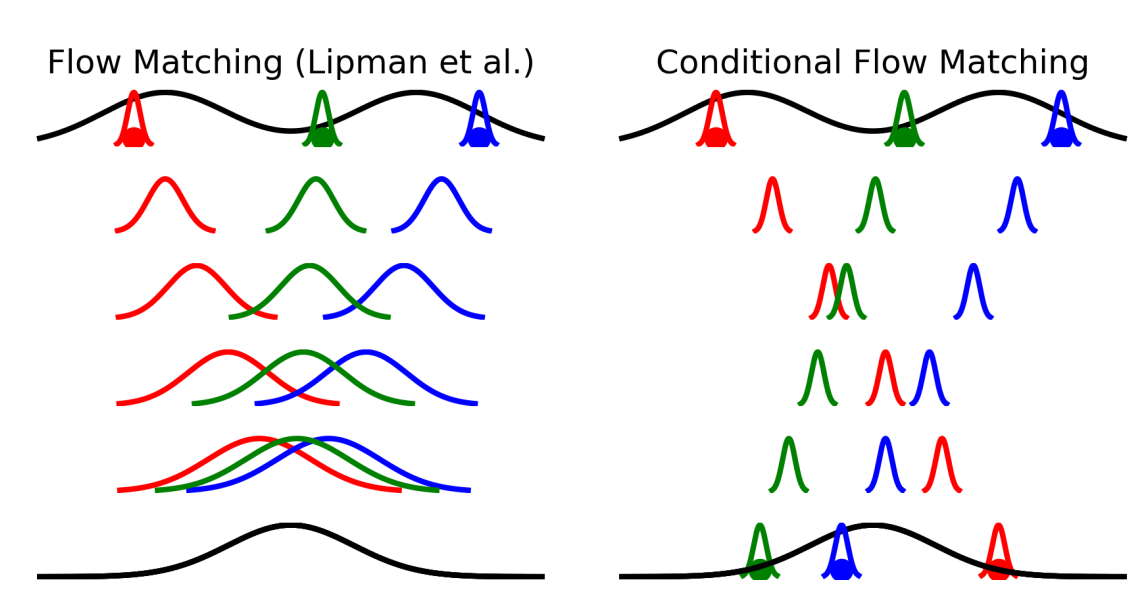
\includegraphics[width=\linewidth]{figs/compare_conditionings}
	\end{figure}
	\myfootnotewithlink{https://arxiv.org/pdf/2302.00482}{Tong A., et al. Improving and Generalizing Flow-Based Generative Models with Minibatch Optimal Transport, 2023}
\end{frame}
%=======
\subsection{Rectified flows}
%=======
\begin{frame}{Rectified flows}
	\begin{figure}
		\centering
		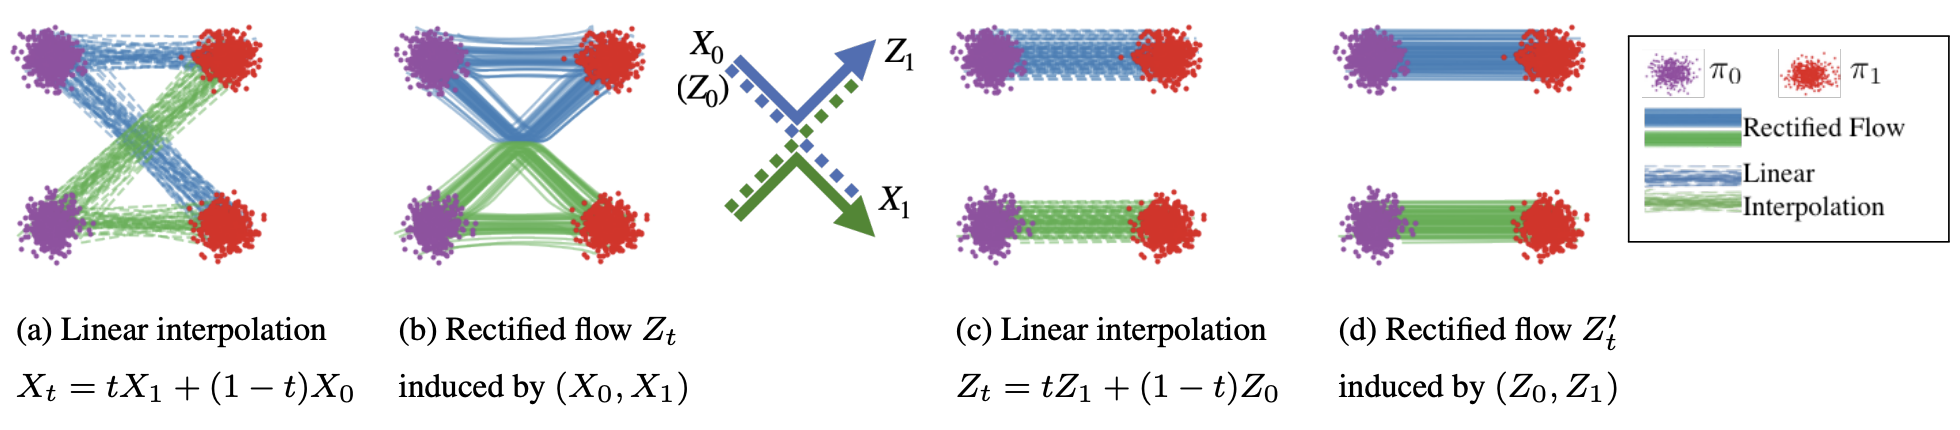
\includegraphics[width=\linewidth]{figs/rectified_flow}
	\end{figure}
	\begin{figure}
		\centering
		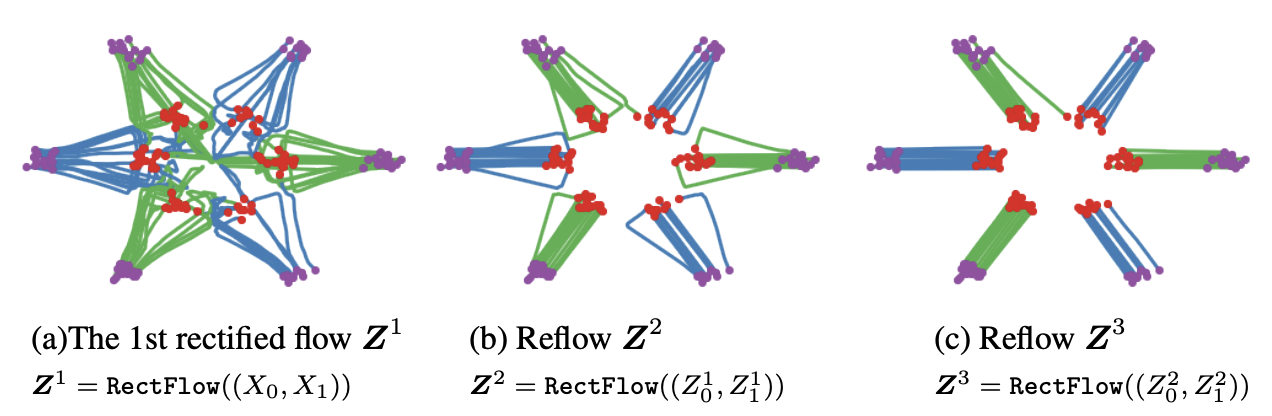
\includegraphics[width=\linewidth]{figs/star_fig}
	\end{figure}
	\myfootnotewithlink{https://arxiv.org/abs/2209.03003}{Liu X., et al. Flow Straight and Fast: Learning to Generate and Transfer Data with Rectified Flow, 2022}
\end{frame}
%=======
\begin{frame}{Rectified flows}
	\begin{figure}
		\centering
		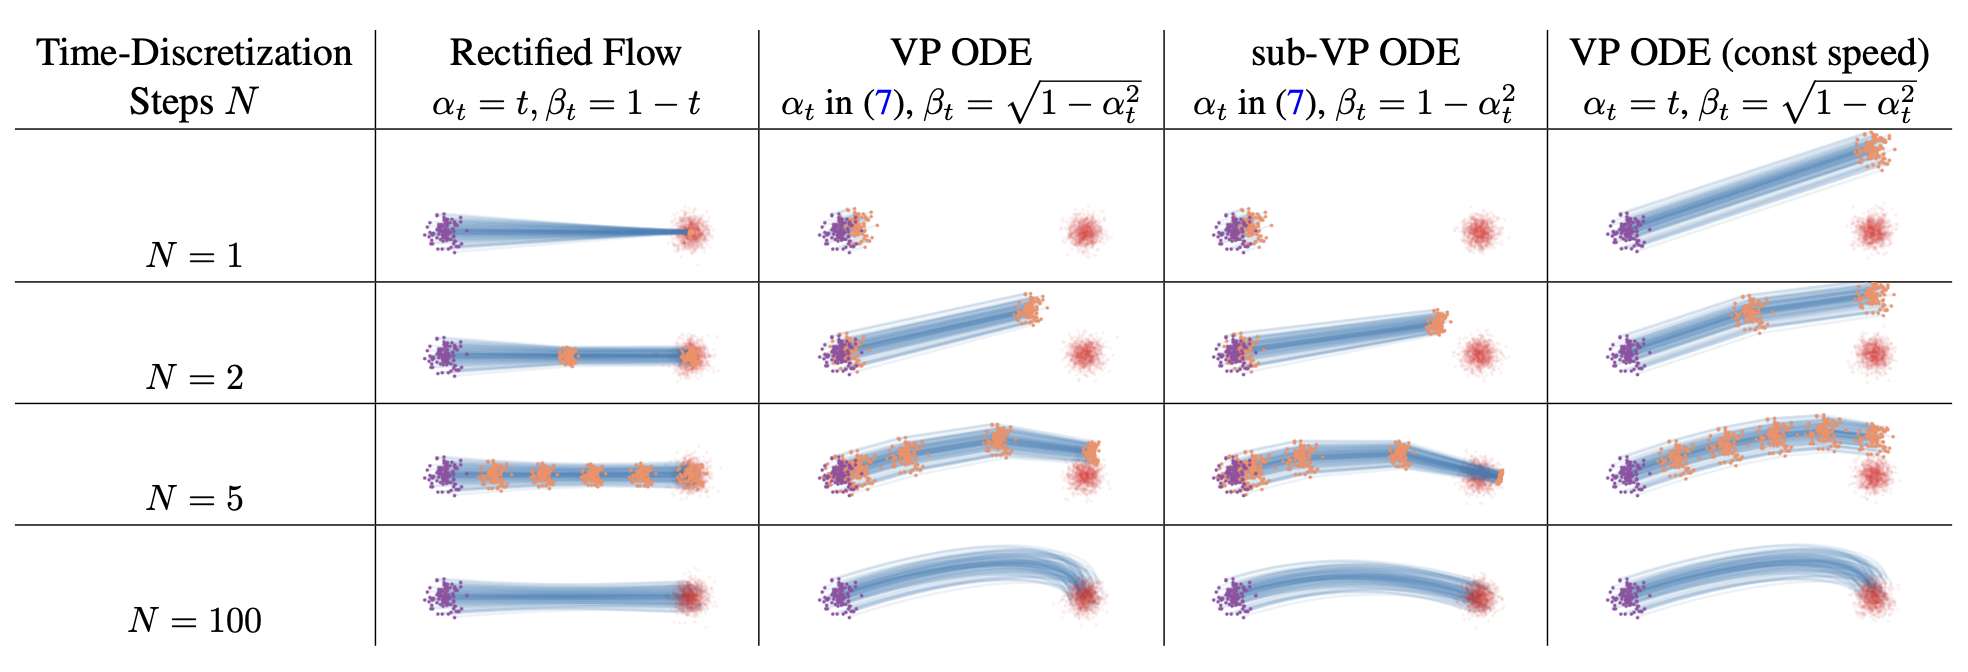
\includegraphics[width=\linewidth]{figs/combined_vp}
	\end{figure}
	\myfootnotewithlink{https://arxiv.org/abs/2209.03003}{Liu X., et al. Flow Straight and Fast: Learning to Generate and Transfer Data with Rectified Flow, 2022}
\end{frame}
%=======
\begin{frame}{Rectified flows}
	\begin{figure}
		\centering
		\includegraphics[width=\linewidth]{figs/sd3}
	\end{figure}
	\myfootnotewithlink{https://arxiv.org/pdf/2403.03206}{Esser P., et al. Scaling Rectified Flow Transformers for High-Resolution Image Synthesis, 2024}
\end{frame}
%=======
\section{Latent models}
%=======
\subsection{Score-based models}
%=======
\begin{frame}{Latent models}
	\begin{figure}
		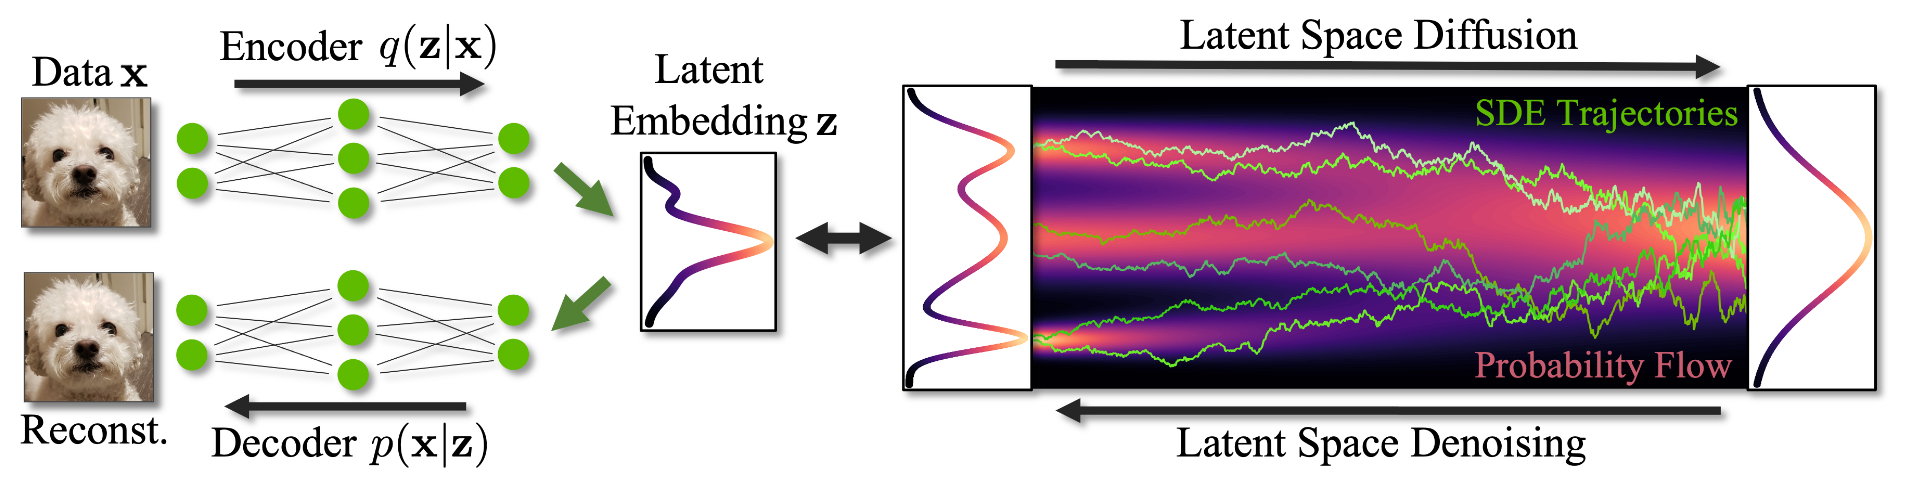
\includegraphics[width=\linewidth]{figs/latent_diffusion}
	\end{figure}
	\begin{figure}
		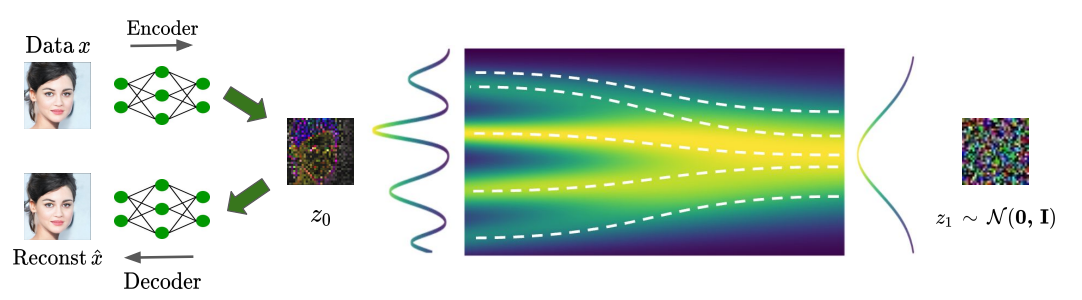
\includegraphics[width=\linewidth]{figs/latent_flow_matching}
	\end{figure}

	\myfootnote{\href{https://arxiv.org/abs/2307.08698}{Dao Q. et al. Flow Matching in Latent Space, 2023} \\ \href{https://neurips2023-ldm-tutorial.github.io/}{NeurIPS 2023 Tutorial: Latent Diffusion Models: Is the Generative AI Revolution Happening in Latent Space?}}
\end{frame}
%=======
\subsection{Autoregressive models}
%=======
\begin{frame}{Vector Quantized VAE (VQ-VAE) }
	\begin{block}{Vector quantization}
		Define the dictionary space $\{\be_k\}_{k=1}^K$, where $\be_k \in \bbR^C$, $K$ is the size of the dictionary.
		\vspace{-0.5cm}
		\begin{minipage}[t]{0.45\columnwidth}
			\[
				\bz_q = \bq (\bz) = \be_{k^*}
			\] 
			Here $k^* = \argmin_k \| \bz - \be_k \|$.
		\end{minipage}%
		\begin{minipage}[t]{0.55\columnwidth}
			\vspace{-0.5cm}
			\begin{figure}
				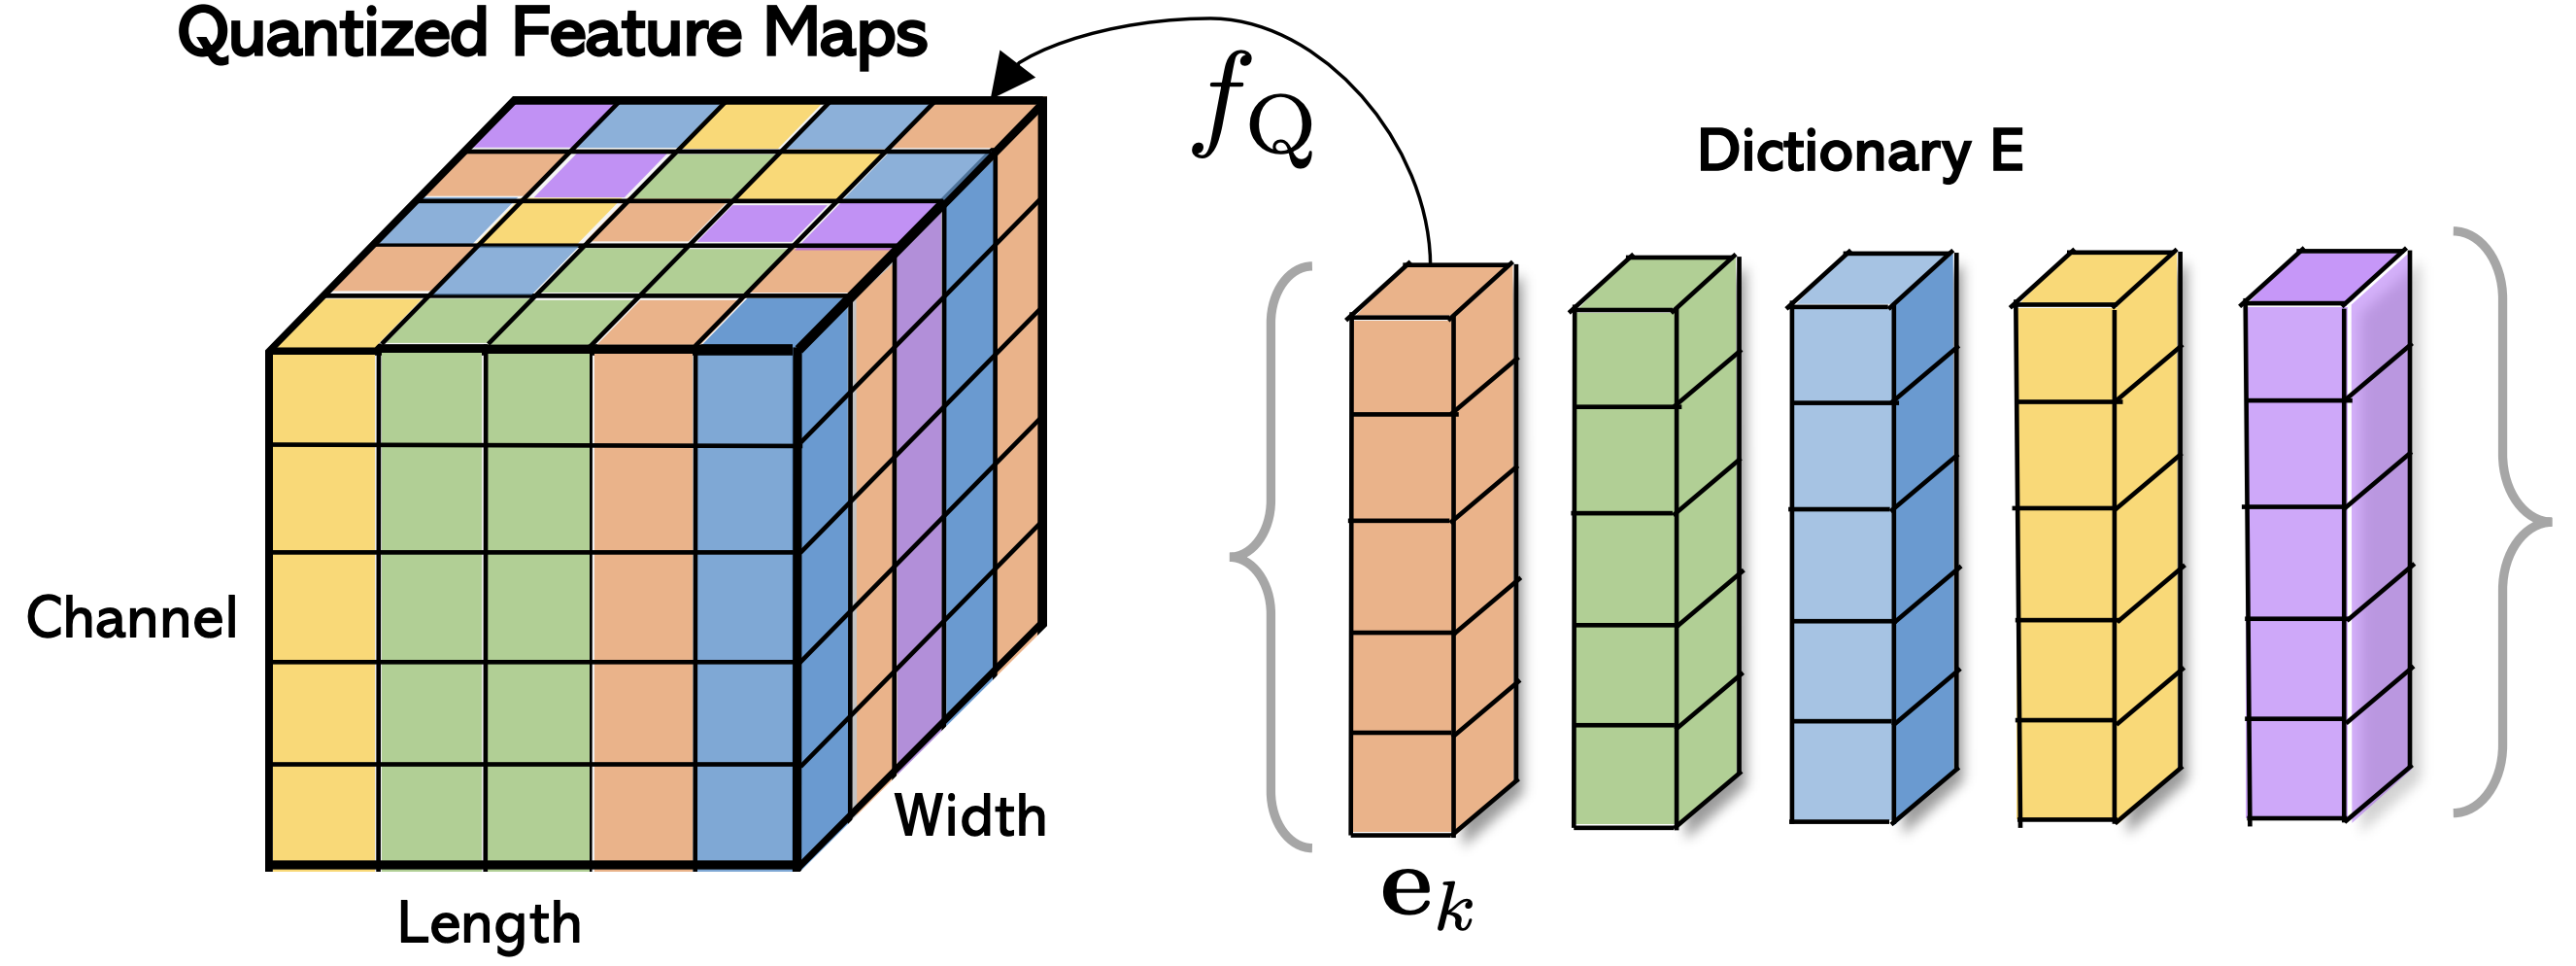
\includegraphics[width=\linewidth]{figs/fqgan_cnn}
			\end{figure}
		\end{minipage}		
	\end{block}
	\[
		\cL_{\bphi, \btheta}(\bx)  =  \log p(\bx | \bz_q, \btheta) - \log K
	\]
	\vspace{-0.5cm}
	\begin{figure}
		\centering
		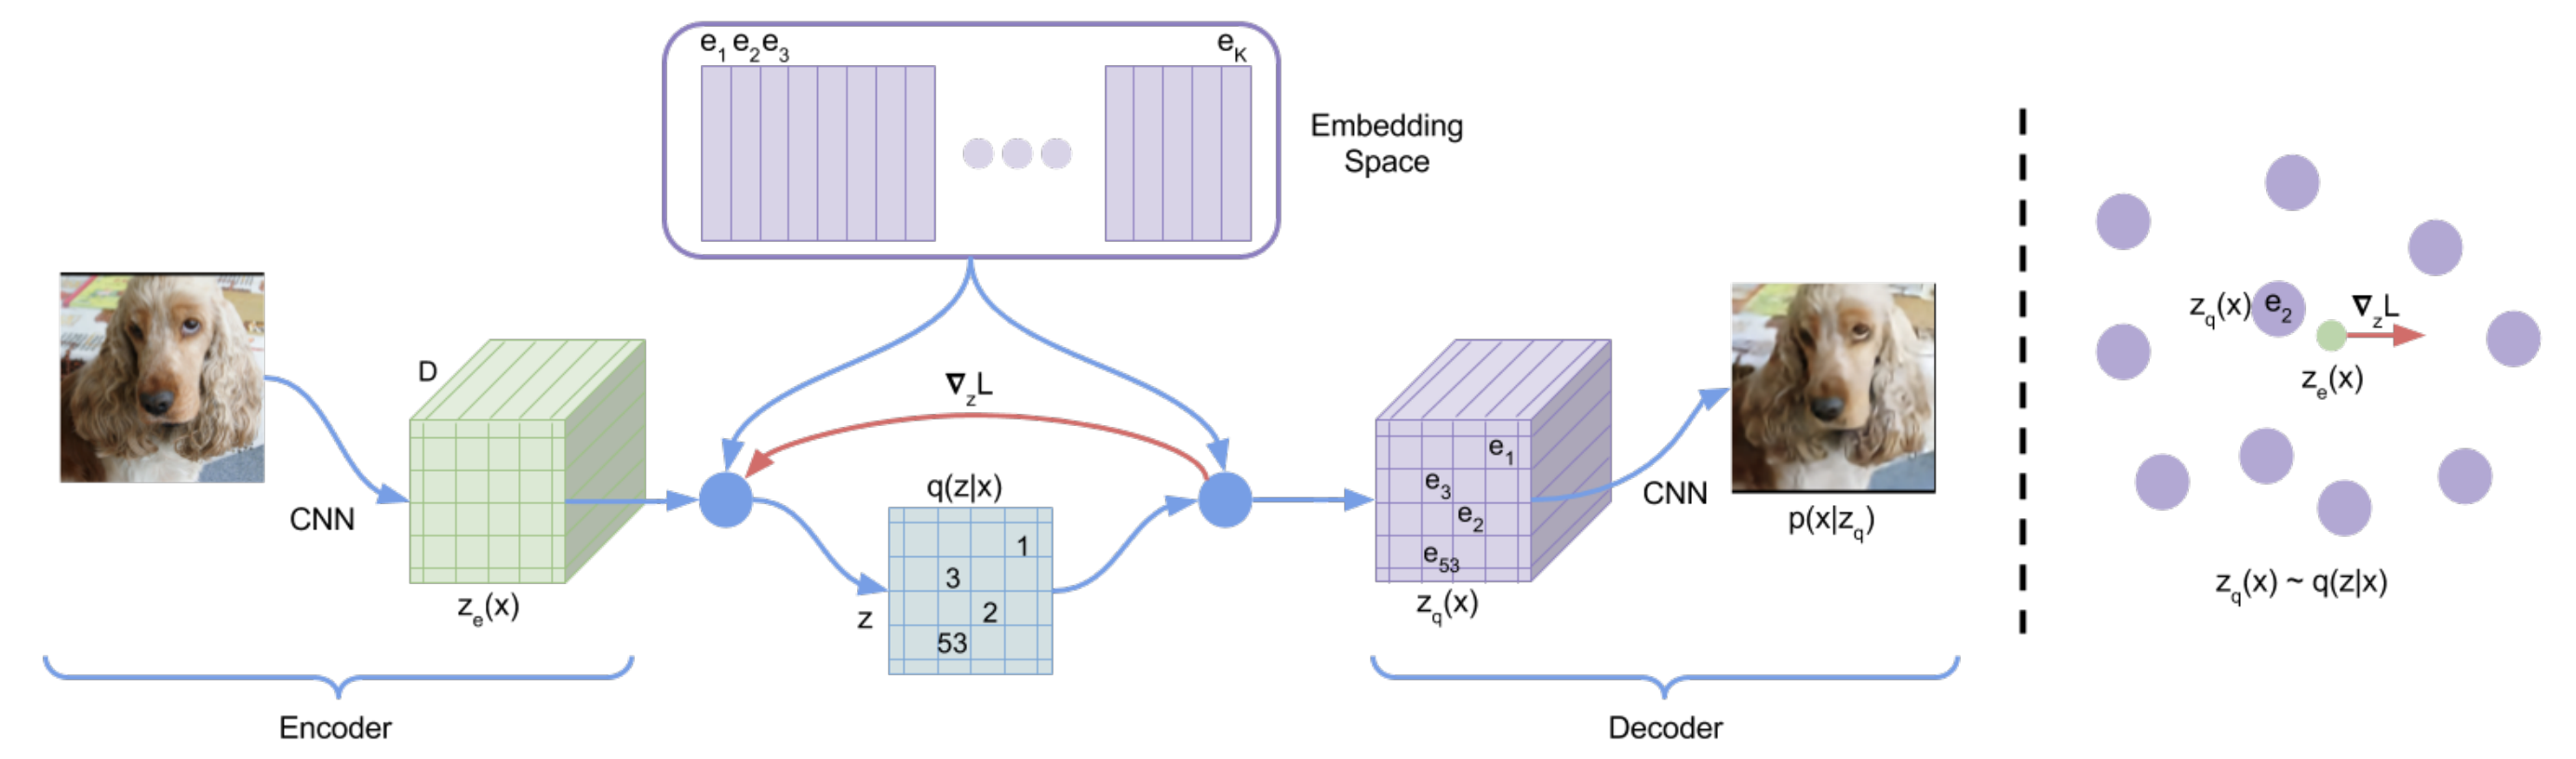
\includegraphics[width=\linewidth]{figs/vqvae}
	\end{figure}
	\myfootnote{\href{https://arxiv.org/abs/2004.02088}{Zhao Y. et al. Feature Quantization Improves GAN Training, 2020} \\ \href{https://arxiv.org/abs/1711.00937}{Oord A., Vinyals O., Kavukcuoglu K. Neural Discrete Representation Learning, 2017}}
\end{frame}
%=======
\begin{frame}{Vector Quantized GAN}
	\begin{figure}
		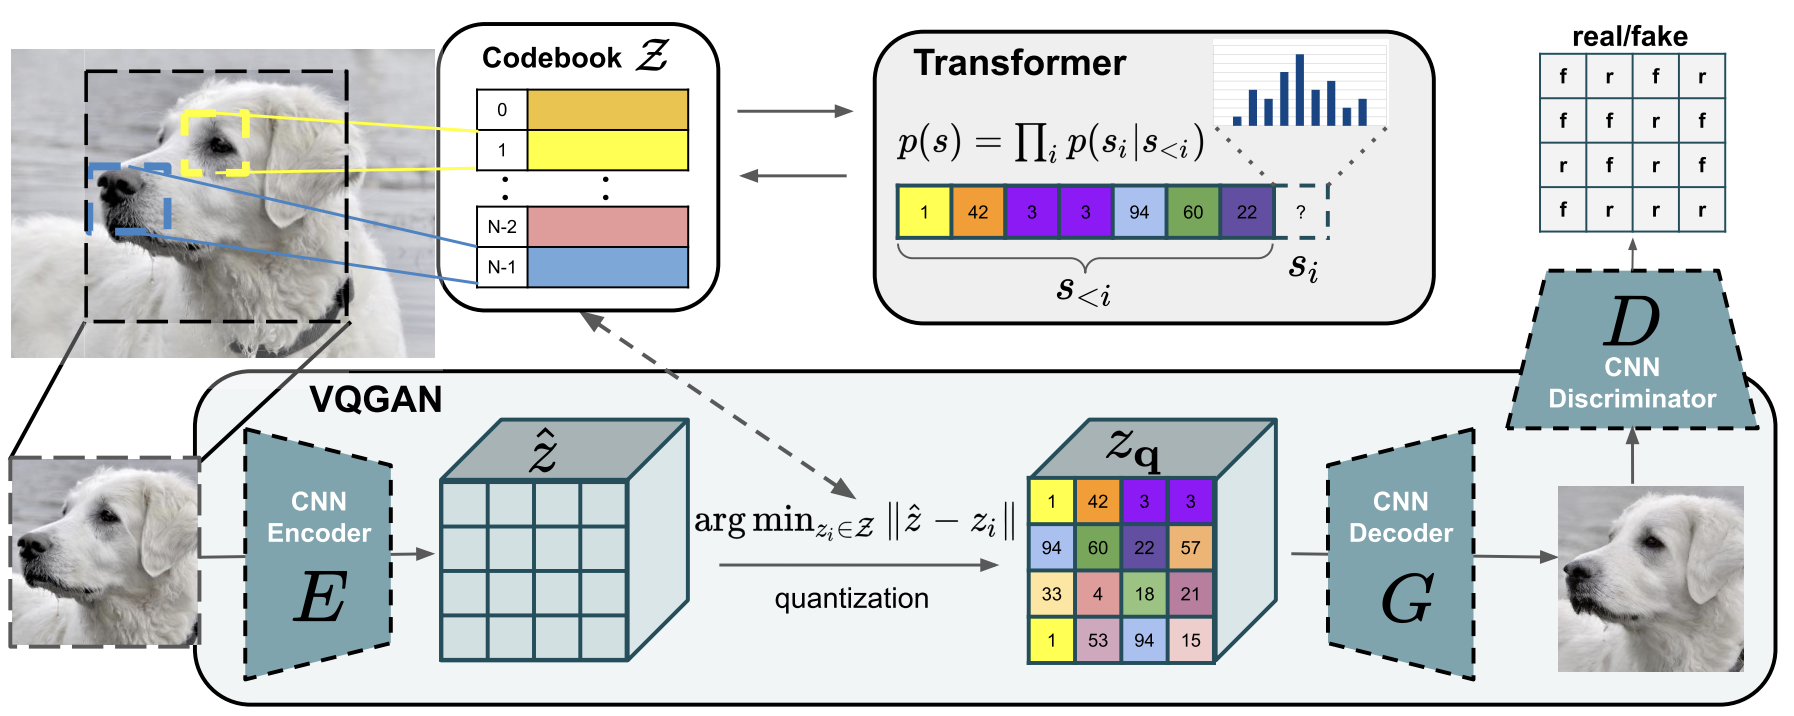
\includegraphics[width=\linewidth]{figs/vqgan}
	\end{figure}
	
	\myfootnotewithlink{https://arxiv.org/abs/2012.09841}{Esser P. et al. Taming Transformers for High-Resolution Image Synthesis, 2020}
\end{frame}
%=======
\begin{frame}{LlamaGen}
	\begin{figure}
		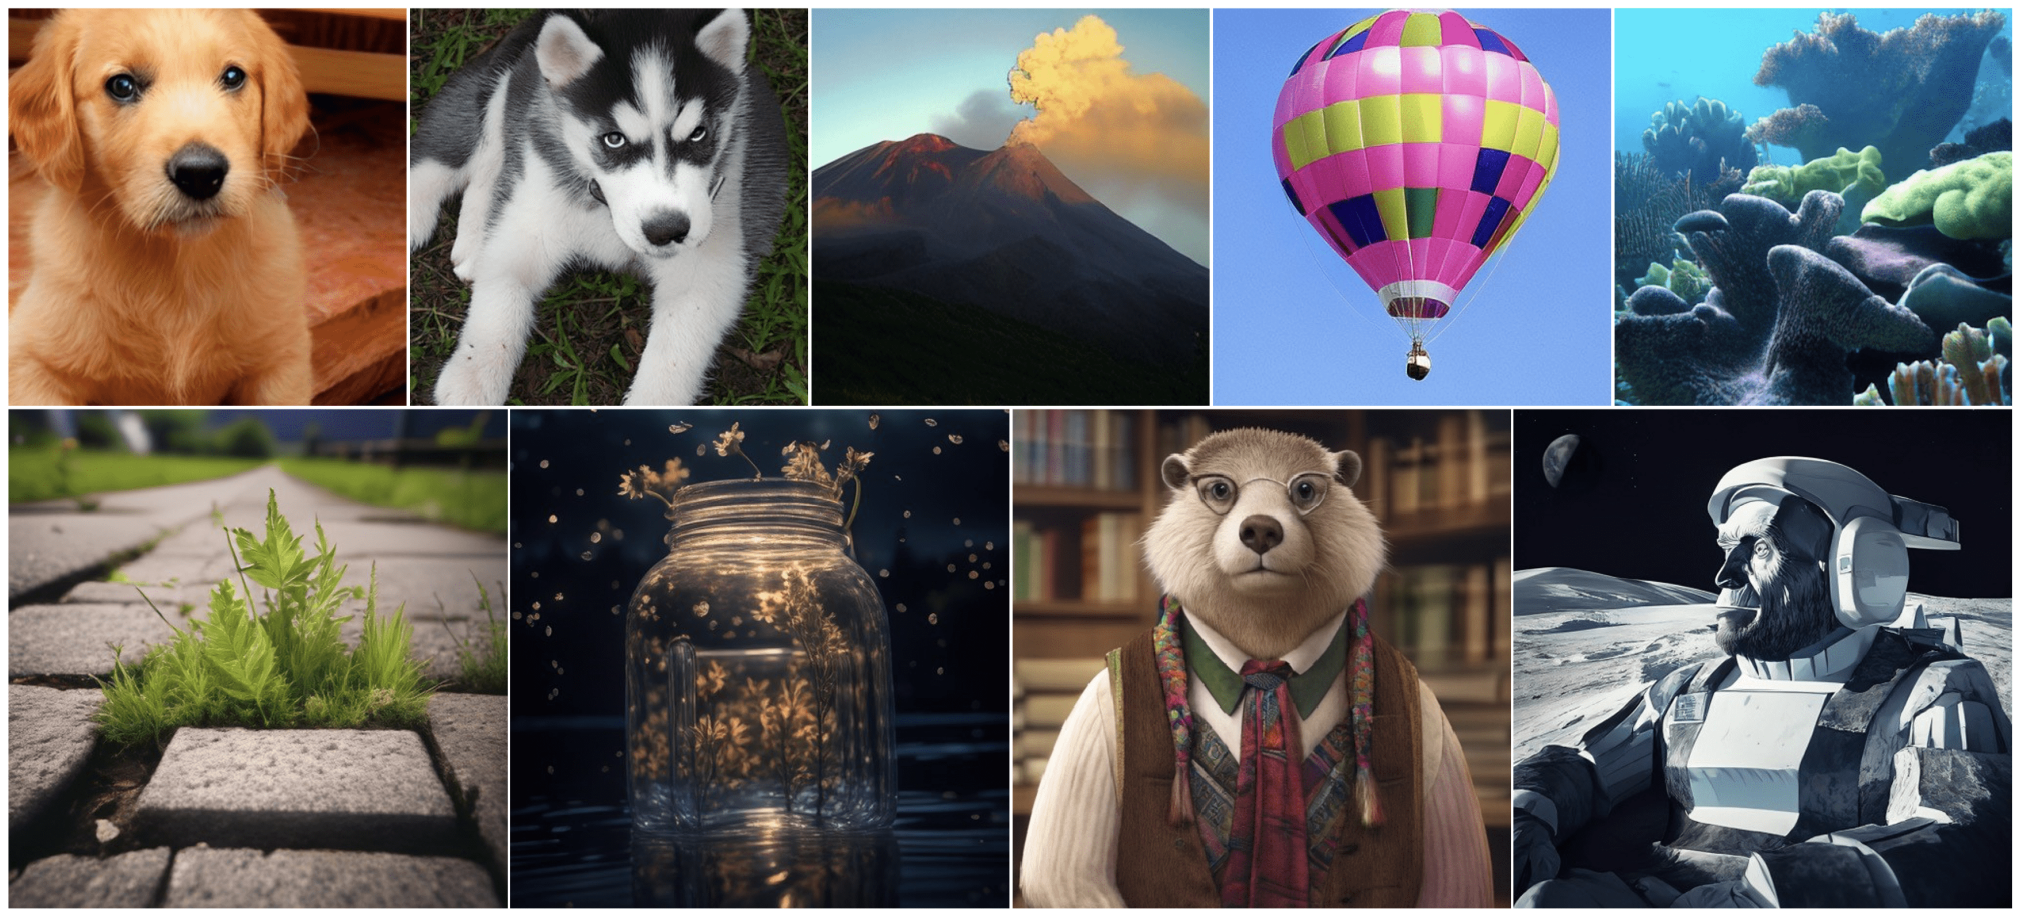
\includegraphics[width=\linewidth]{figs/llamagen_samples}
	\end{figure}
	
	\myfootnotewithlink{https://arxiv.org/pdf/2406.06525}{Sun P. et al. Autoregressive Model Beats Diffusion: Llama for Scalable Image Generation, 2024}
\end{frame}
%=======
\begin{frame}{Visual Autoregressive Modeling (VAR)}
	\begin{figure}
		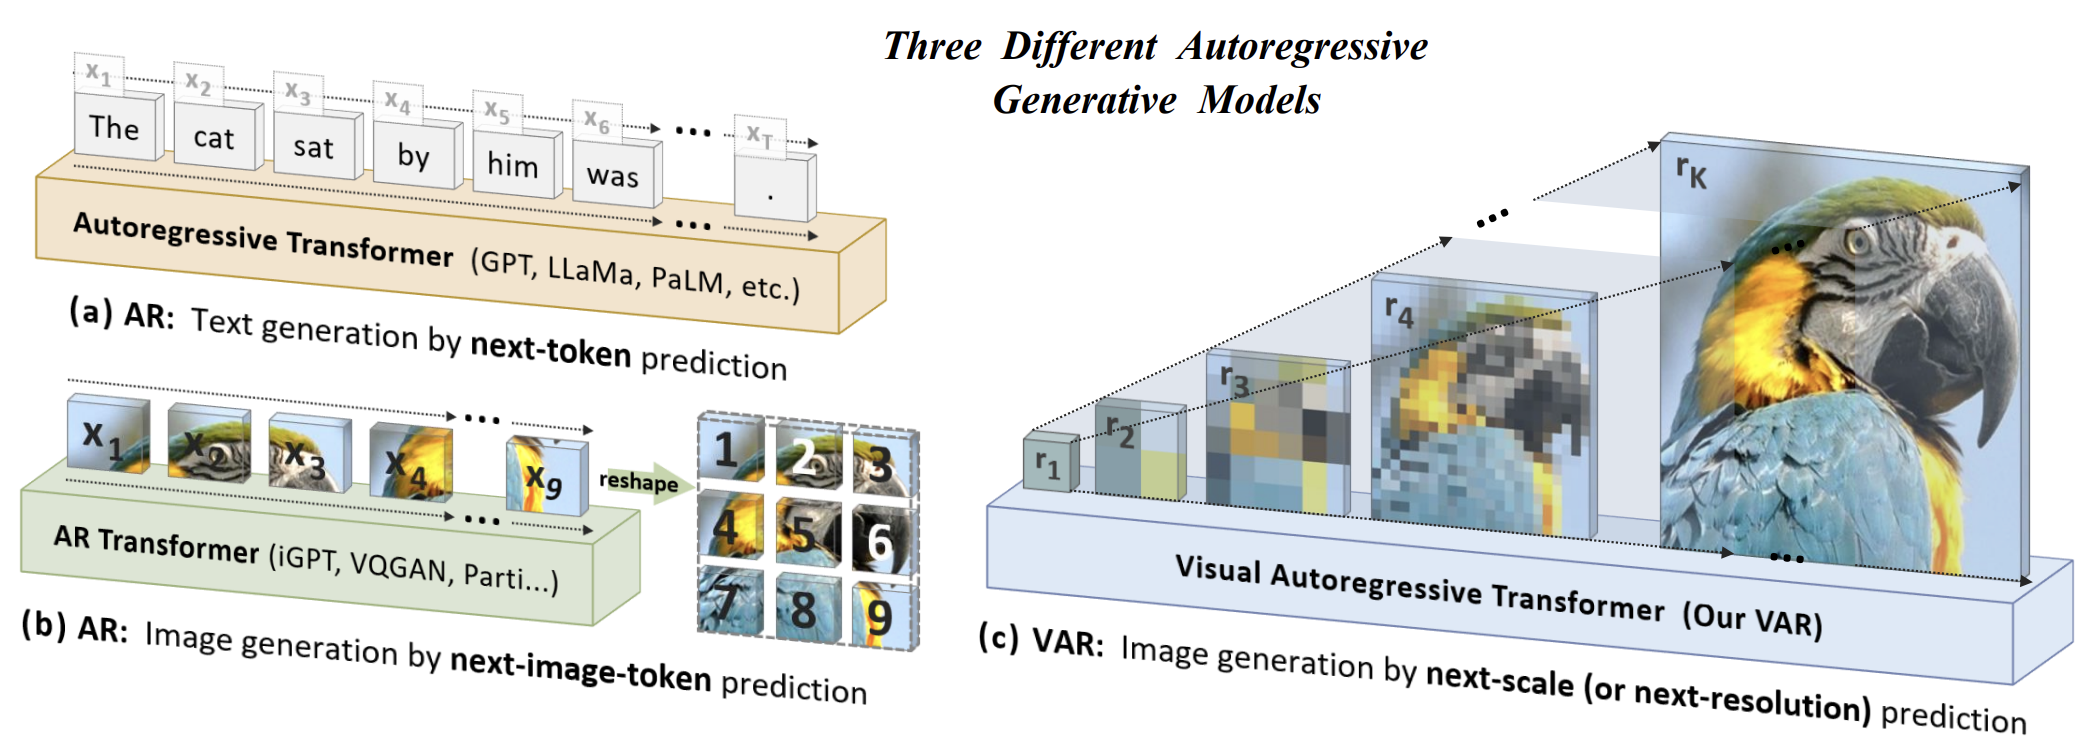
\includegraphics[width=\linewidth]{figs/var_idea}
	\end{figure}
	
	\myfootnotewithlink{https://arxiv.org/pdf/2404.02905}{Tean K. et al. Visual Autoregressive Modeling: Scalable Image Generation via Next-Scale Prediction, 2024}
\end{frame}
%=======
\begin{frame}{Visual Autoregressive Modeling (VAR)}
	\begin{figure}
		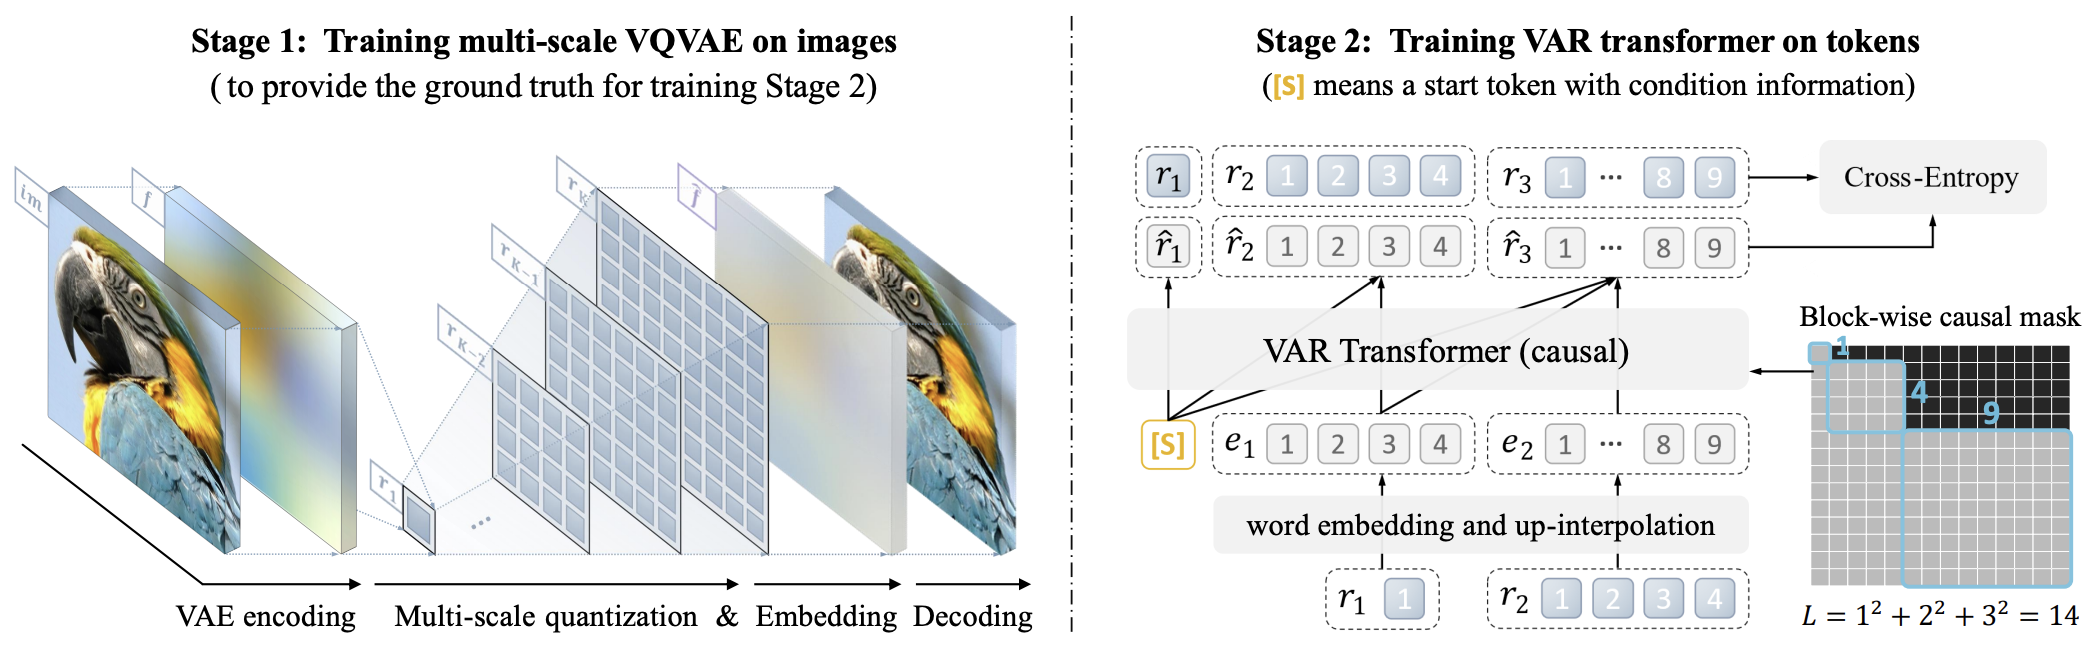
\includegraphics[width=\linewidth]{figs/var_training}
	\end{figure}
	
	\myfootnotewithlink{https://arxiv.org/pdf/2404.02905}{Tean K. et al. Visual Autoregressive Modeling: Scalable Image Generation via Next-Scale Prediction, 2024}
\end{frame}
%=======
\section{The worst course overview}
%=======
\begin{frame}{The worst course overview :)}
	\begin{figure}
		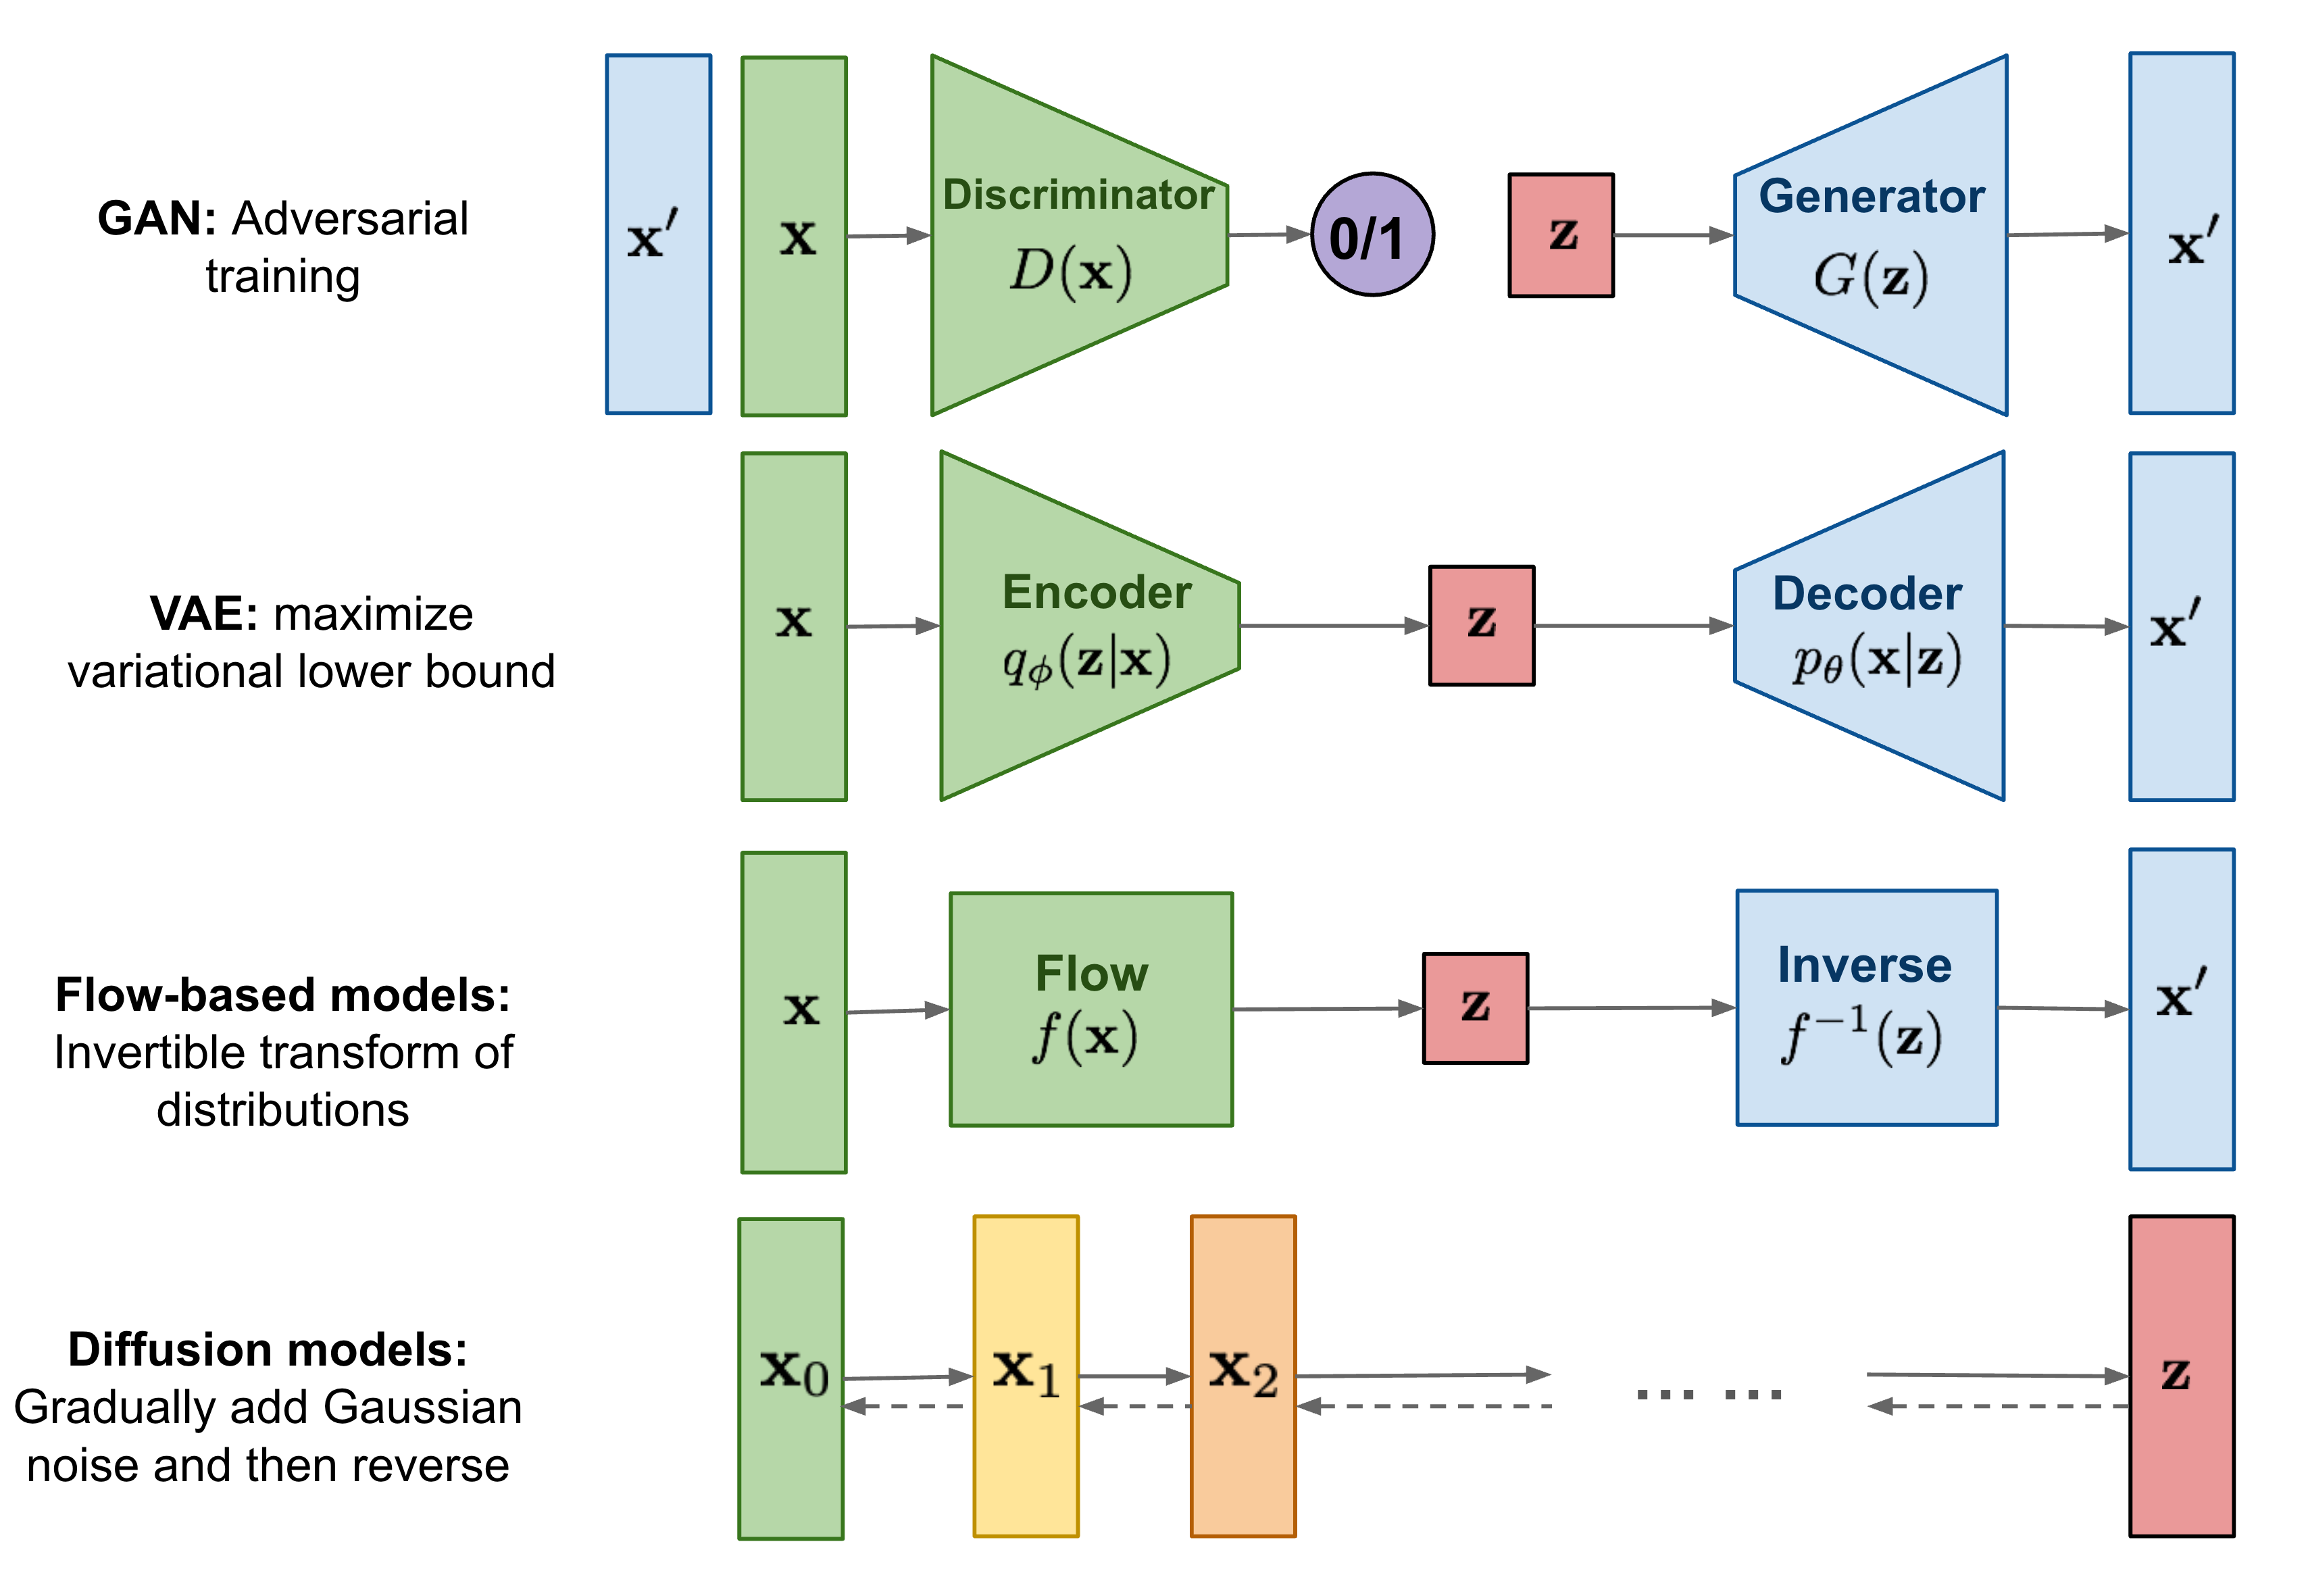
\includegraphics[width=\linewidth]{figs/generative-overview}
	\end{figure}
	\myfootnotewithlink{https://lilianweng.github.io/posts/2021-07-11-diffusion-models/}{Weng L. What are Diffusion Models?, blog post, 2021}
\end{frame}
%=======
\begin{frame}{The worst course overview :)}
	\begin{figure}
		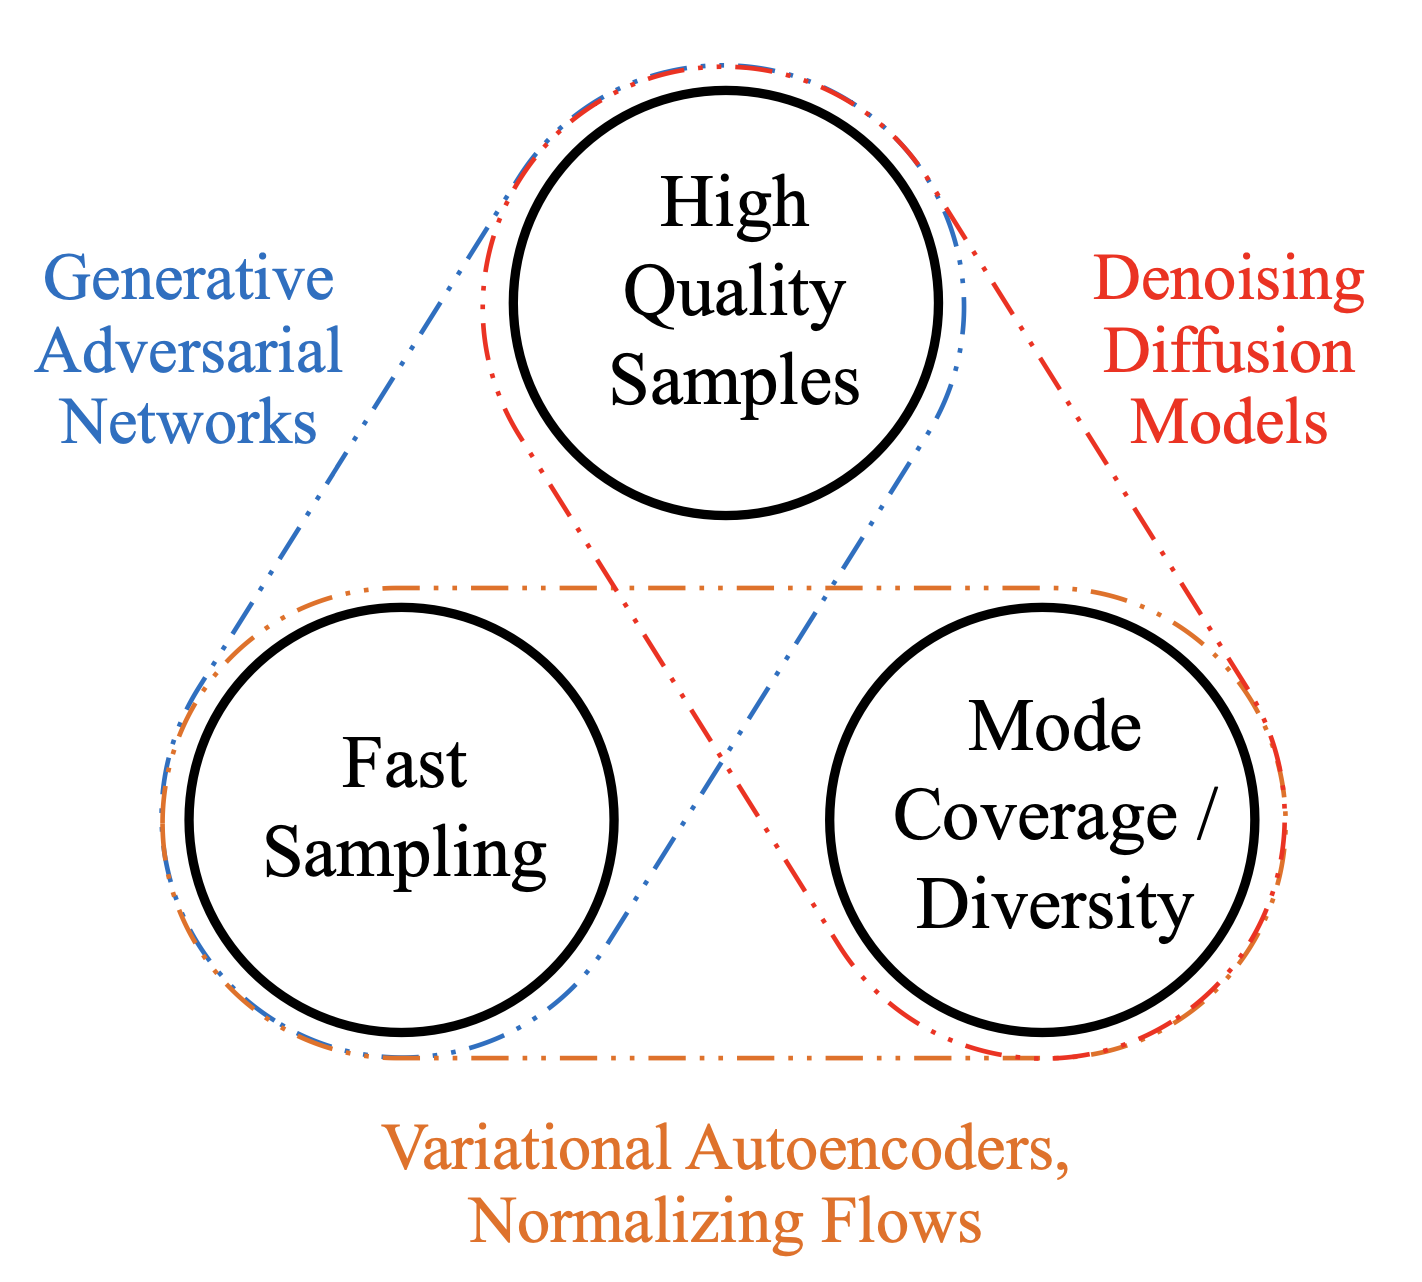
\includegraphics[width=0.7\linewidth]{figs/trilemma}
	\end{figure}
	\myfootnotewithlink{https://arxiv.org/abs/2112.07804}{Xiao Z., Kreis K., Vahdat A. Tackling the generative learning trilemma with denoising diffusion GANs, 2021}
\end{frame}
%=======
\begin{frame}{The worst course overview :)}
	\begin{figure}
		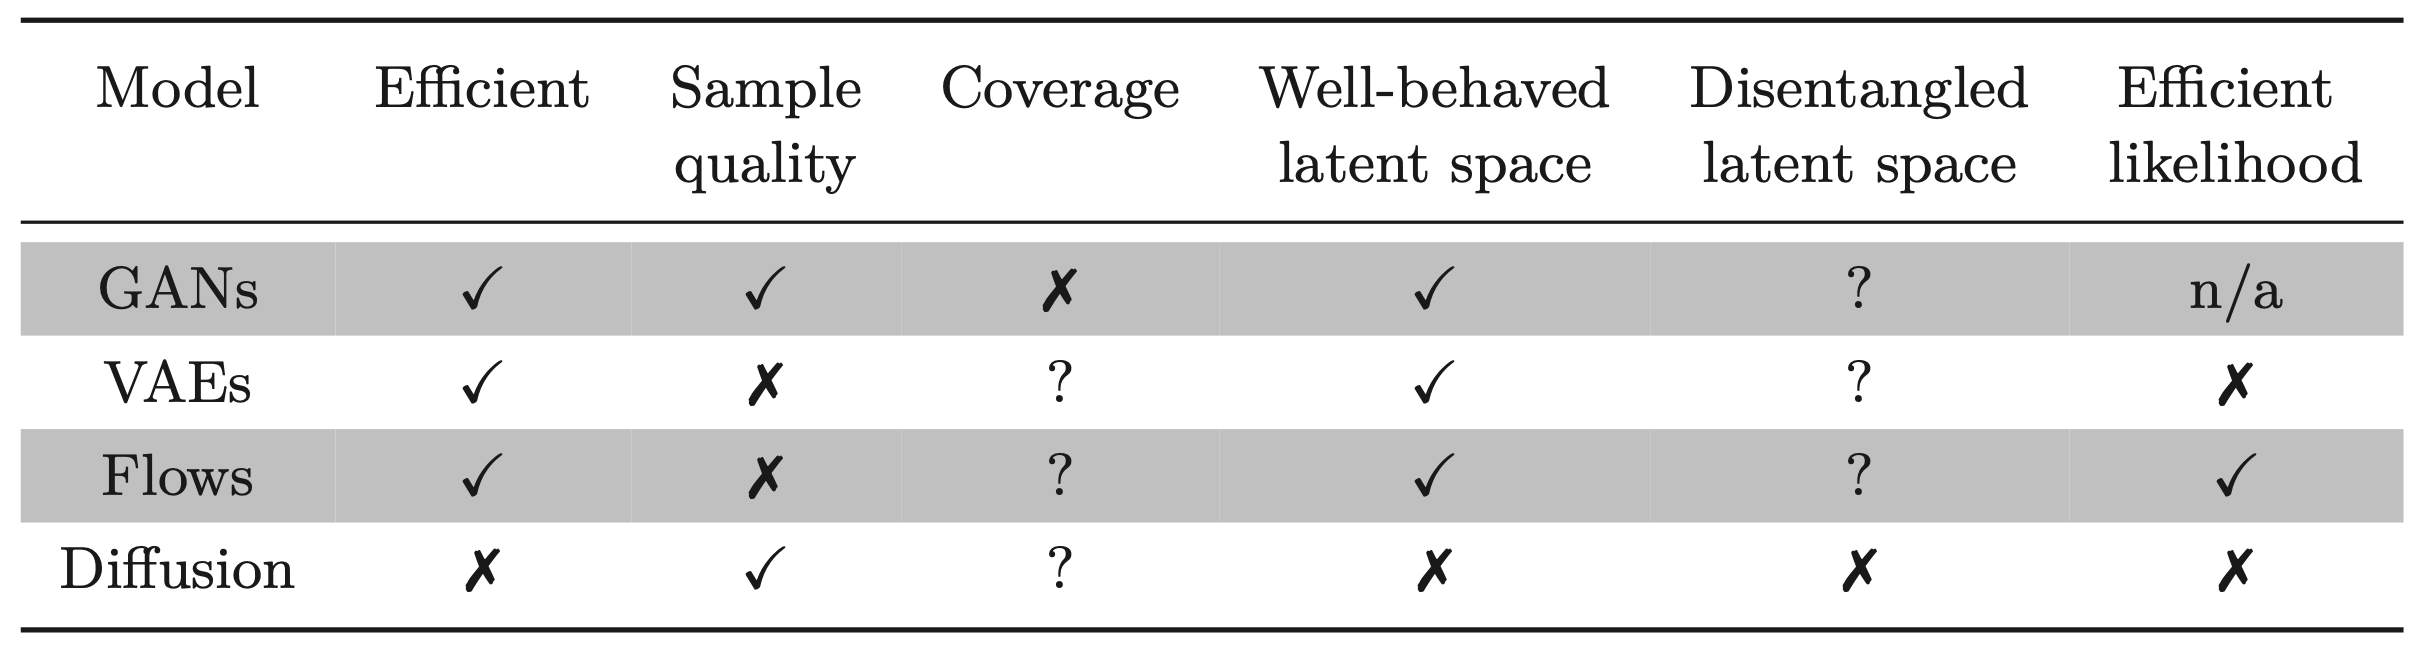
\includegraphics[width=\linewidth]{figs/gen_comp_table}
	\end{figure}
	\myfootnotewithlink{https://udlbook.github.io/udlbook/}{Simon J.D. Prince. Understanding Deep Learning, 2023}
\end{frame}
%=======
\begin{frame}{Summary}
	\begin{itemize}
		\item 
	\end{itemize}
\end{frame}
\end{document} 